\documentclass[conference]{IEEEtran}
\IEEEoverridecommandlockouts
% The preceding line is only needed to identify funding in the first footnote. If that is unneeded, please comment it out.
\usepackage{cite}
\usepackage{amsmath,amssymb,amsfonts}
\usepackage{algorithmic}
% \usepackage{algorithm}
\usepackage[ruled]{algorithm2e}
\usepackage{graphicx}
\usepackage{textcomp}
\usepackage{xcolor}
\usepackage{multirow}
\def\BibTeX{{\rm B\kern-.05em{\sc i\kern-.025em b}\kern-.08emT\kern-.1667em\lower.7ex\hbox{E}\kern-.125emX}}
\setcounter{secnumdepth}{4}
\begin{document}

\title{\huge IoT-Based Opioid Overdose Monitoring System\\
{\LARGE CPSC 503.08 Final Report}
% \thanks{Identify applicable funding agency here. If none, delete this.}
}

\author{\IEEEauthorblockN{Jian Liao}
\IEEEauthorblockA{\textit{Department of Computer Science} \\
\textit{University of Calgary}\\
Calgary AB, Canada \\
jian.liao1@ucalgary.ca}
\and
\IEEEauthorblockN{Advisor: Dr. Mea Wang}
\IEEEauthorblockA{\textit{Department of Computer Science} \\
\textit{University of Calgary}\\
Calgary AB, Canada \\
meawang@ucalgary.ca}
}

\maketitle

\begin{abstract}
The opioid epidemic in Canada has claimed the lives of over 8000 people in the last two years, and everyday 11 people die from an opioid overdose. This problem is clearly not improving, and it is urgently addressed that many individuals are trying to find a solution to opioid crisis. Fortunately, the Internet of Things (IoT) has provided a promising opportunity to tackle the opioid epidemic challenge. Therefore, with the use of IoT, this paper will try to explore a solution and implement an opioid overdose monitoring system with the goals of achieving high sclability and real-time services.
\end{abstract}

\begin{IEEEkeywords}
Opioid overdose, health monitoring, Internet of Things (IoT), IoT database, cloud computing, data visualization
\end{IEEEkeywords}

\section{Introduction}
Over the past two decades, the United States population has experienced an extraordinary increase in the rates of death from opioid overdose. A steep rise in fatal overdoses caused by pharmaceutical opioids observed over the last 15 years \cite{b1} has been overtaken by rapidly increasing rates of heroin and illicit fentanyl overdose death as the supply of prescription opioids has been reduced \cite{b2}. In 2017, there were estimated to be 68,400 drug overdose deaths in the US \cite{b3}, more than the annual number of deaths from AIDS at the height of that epidemic. These deaths have contributed to an overall decrease in life expectancy among middle-aged white people in the US \cite{b4}. Another report in 2018 shows that every day, 128 people in the United States die after overdosing on opioids \cite{b5}. The misuse of and addiction to opioids, including prescription pain relievers, heroin, and synthetic opioids such as fentanyl, which is a serious national crisis that affects public health as well as social and economic welfare. Meanwhile in Canada, the opioid epidemic has claimed the lives of over 8000 people in the past two years, and has resulted in 11 opioid overdose related deaths every day \cite{b6}. Of those deaths, almost 70\% involved a prescription or illicit opioid.

The government of Canada is committed to fighting the opioid overdose epidemic and supporting states and communities as they continue work to identify outbreaks, collect data, respond to overdoses, provide care to those in their communities, and set up supervised consumption sites all over Canada for surveillance and prevention efforts \cite{b7}. These efforts include timelier tracking of nonfatal and fatal drug overdoses, improving toxicology to better track polysubstance-involved deaths, enhancing linkage to care for people with opioid use disorder and risk for opioid overdose, improving prescription drug monitoring programs, implementing health systems interventions, partnering with public safety, and implementing other innovative surveillance and prevention activities \cite{b8}. However, these federal actions responding to the opioid crisis still encounter a major deficiency which is the increasing requirement for continuous monitoring for the PWUD (People Who Use Drugs) and rapid medical emergency response system in case of opioid overdose occurs \cite{b9}.

To assist the government of Canada in the fight against opioid crisis, it is necessary to propose a more efficient, and practical approach to tackling the problem. Originally, I teamed up in the Innovation4Health program and we proposed the idea of the opioid overdose monitoring system. And based on the previous work, this research project proposes a more satisfactory solution which is to develop an IoT-based opioid overdose monitoring system that is capable of automatically collecting and transmitting vital signs data (heart rate and respiration rate) using existing sensor solutions (ECG), storing and analyzing the data on the IoT cloud data platform to detect opioid overdose, and alerting a medical emergency so that the patients can get the rapid medical care they need. This proposed IoT-based opioid overdose monitoring system consists of 5 components in general. 

First, the monitoring module (IoT device) will be composed of several physiological sensors and communication modules such as Electrocardiography sensor, accelerometer, and Bluetooth Low Energy 4.0 module. Second, a cross-platform technique (Dart \& Flutter) will be used to develop the end-user mobile application layer. Third, IoT Middleware layer is implemented using MQTT protocol (Broker) as a gateway, which provides a medium for the communication between the edge device and the back-end server with reliable data transfer (QoS). Fourth, the Web-Tier application will be hosted on the server with different services implemented using Node.js \cite{ref5}. These services include synchronizing and managing the gateway systems, transmitting data to and from the IoT data platform, handling all the requests and send it back to the requester. Fifth, the IoT data platform consists of two parts, cloud data engine (scientific computation module \& cloud database) and microservices. The cloud data engine contains a scientific computation module and cloud database which can store the sensor data and perform specific computation tasks on the sensor data. 

% The advantage of using such an environment is that it ensures the cross-platform feature for application which means that only one application is developed for different mobile phone platforms without the need for reimplementation. The mobile application will allow end-user to check on the status as well as the readings of the sensors which are connected through BLE.

% On the broker side, access control is enforced to prevent unauthorized access to certain topics. Also, broker server can be highly scalable to maintain high concurrency of connections. 

% Moreover, a dashboard application will be provided that allows users to operate specific tasks such as device control and performance analytics.

% The microservices will be implemented between the cloud data engine and web-tier application (back-end). The cloud data engine contains a scientific computation module and cloud database which can store the sensor data and perform specific computation tasks on the sensor data. 
% For instance, execute machine learning algorithms to analyse the sensor data to see if opioid overdose occurs.

The modules other than the IoT data platform in the system have been developed outside of this course and the goal of this research project is to develop the cloud-based IoT data platform. The overview of the IoT data platform in terms of technologies includes communication protocols design (MQTT \& RESTful API), cloud database design, highly scalable broker server design (Load Balancer) and real-time data processing \& visualization (Data Driven Document). And the expected outcome in terms of functionality and performance of this research project is to provide a full-featured ecosystem as well as the cloud IoT data platform, seamless sync from edge to cloud, guaranteed data availability, high scalability and real-time services. And for the rest of this paper, we will review related work in Sec. \uppercase\expandafter{\romannumeral2}, and propose the design of the IoT data platform in Sec. \uppercase\expandafter{\romannumeral3}.  The evaluation of the platform is presented in Sec. \uppercase\expandafter{\romannumeral4}, followed by conclusion in Sec. \uppercase\expandafter{\romannumeral5}.

% You can extend this part to overview the technologies that you will use to develop this platform and the goals (e.g., scalable database server, real-time data visualization).  The goals will be the things that you will measure in the evaluation section.



\section{Related Work}
% This section will introduce related work and researches on IoT management system. 
The Internet of Things is an emerging technology which is generally recognized as representing a revolution in Information and Communication Technology (ICT). It is expected to have a wide range of applications in various industrial sectors, including healthcare \cite{ref6,ref7} and energy industry \cite{ref8}. According to research on IoT-based healthcare asset management system (IoT-HAMS), a general system architecture of IoT-HAMS is proposed \cite{ref9}. The system components include RFID and Wireless Sensor Network (WSN) devices (IoT devices), IoT middle‐ware, graphic user interface (GUI) for rules input and modification, cloud database, and core management engine. This state-of-the-art provides a very specific solution stack for IoT-HAMS which shares several similarities to the solution this paper is proposing such as IoT devices, IoT middle-ware layer, cloud database and GUI applications. However, what differs from IoT-HAMS is that our solution guarantees data reliability as well as instantaneity and focuses more on establishing a highly sclable system that is capable of performing specific data processing tasks on the real-time input data while IoT-HAMS focuses more on devices management.

% Another research presents an IoT-based home energy management systems (IoT-HEMS), a three-layer system architecture \cite{ref10}. This system composes of Hardware layer (sensors, actuators and high-end microcontroller), Software layer (data acquisition module and middleware module) and Client application layer. This research states a specific solution to HEMS with more interests in hardware implementation and data integrity while IoT Manager concentrates on providing a full-featured ecosystem as well as a one-stop service from edge to cloud and performing data processing tasks on the fly.

Amazon (AWS), Microsoft (Azure) and Google also provide the state-of-the-art IoT platfrom solution for industrial, consumer and commercial use. The AWS IoT is the leader in IoT in terms of the number of services provided. AWS IoT solutions are available for both edge software and cloud services. Edge software allows developers to connect devices, collect data, and perform data analysis. Whereas, the AWS Cloud Services enable them to securely connect a group of devices, manage the devices, keep them secure, and detect, and respond to IoT events across IoT apps and sensors. The Azure IoT is a collection of cloud services that connect, monitor, and control billions of IoT assets which is managed by Microsoft. It is the second-largest IoT platform in terms of the market share. The IoT solution is made up of one or more IoT devices and one or more back-end services running in the cloud which communicate with each other. There are two paths for building the solution which are Platform as a Service (PaaS) and Software as a Service (SaaS). The Google IoT is one of the top IoT service providers around the world, making it easier for developers to build connected devices. It provides Cloud IoT Core as its flagship IoT solution for creating secure and innovative solutions. In details, the comparison of these solutions is as shown in Table \ref{tab:iot-services}. All of these state-of-the-art IoT platform solutions share advanced and well-established techniques in terms of cloud services, data storage, cloud computation and key tools. What differs from our solution is that while these industrial solutions focus more on the breadth of provided IoT services for multiple scenarios, our solution explore the depth of the IoT health monitoring solution with high scalability and real-time services. However, these solutions have inspired and set the goal standard of the implementation and evaluation in this paper.

% The Azure IoT solution accelerators include a collection of PaaS solutions that we can use to accelerate our development of an IoT solution. And the Azure IoT Central is a SaaS solution that helps us connect, monitor, and manage the IoT devices.

% Please add the following required packages to your document preamble:
% \usepackage{multirow}
\begin{table}[htbp]
\centering
\caption{IoT Platform Solutions Comparison}
\label{tab:iot-services}
\begin{tabular}{|c|l|c|c|c|}
\hline
\multicolumn{2}{|c|}{\multirow{2}{*}{\textbf{\begin{tabular}[c]{@{}c@{}}IoT\\ Solution\end{tabular}}}} &
  \multicolumn{3}{c|}{\textbf{IoT Platform Solution Provider}} \\ \cline{3-5} 
\multicolumn{2}{|c|}{} &
  \textbf{AWS} &
  \textbf{Azure} &
  \textbf{Google} \\ \hline
\multicolumn{2}{|c|}{Services} &
  \begin{tabular}[c]{@{}c@{}}AWS Web Services\\ AWS Cloud Services\end{tabular} &
  \begin{tabular}[c]{@{}c@{}}Azure PaaS\\ Azure SaaS\end{tabular} &
  \begin{tabular}[c]{@{}c@{}}Google Cloud \\ (IoT Core)\end{tabular} \\ \hline
\multicolumn{2}{|c|}{Protocols} &
  MQTT &
  \begin{tabular}[c]{@{}c@{}}HTTP\\ MQTT\\ AMQP\end{tabular} &
  \begin{tabular}[c]{@{}c@{}}HTTP\\ MQTT\end{tabular} \\ \hline
\multicolumn{2}{|c|}{Storage} &
  Elastic Block Storage &
  Blob Storage &
  Cloud Storage \\ \hline
\multicolumn{2}{|c|}{Database} &
  \begin{tabular}[c]{@{}c@{}}Aurora \\ ElastiCache\end{tabular} &
  \begin{tabular}[c]{@{}c@{}}SQL\\ CosmosDB\end{tabular} &
  \begin{tabular}[c]{@{}c@{}}Cloud SQL\\ Cloud Bigtable\end{tabular} \\ \hline
\multicolumn{2}{|c|}{Computation} &
  \begin{tabular}[c]{@{}c@{}}AWS Beanstalk\\ VMware Cloud\\ Serverless Application\end{tabular} &
  \begin{tabular}[c]{@{}c@{}}FaaS\\ Service Fabric\\ Azure Batch\end{tabular} &
  \begin{tabular}[c]{@{}c@{}}App Engine\\ Docker\\ Compute Engine\end{tabular} \\ \hline
\multicolumn{2}{|c|}{Key Tools} &
  IoT Core &
  IoT Hub &
  Cloud IoT Core \\ \hline
\end{tabular}
\end{table}

% Please think about the goals for this development. As I suggested in Sec I, I think it sould be scalable and real-time.  If these are the goals, then your design should serve thiese goals.  If you define other goals, make sure the entire design is consitently serving the same set of goals.  Also, keep in mind that you will be able to evaluate your system against these goals in Sec. IV to show that this project has been successfully developed.

\section{Design}

% (1-2 paragraphs) Overview design of the cloud-based processing platform with a diagram for visual illustration.  Briefly explain each module and their role in this platform.

This research project mainly focuses on the implementation of IoT Data Platform. The goal for the implementation is to develop a real-time and highly scalable system, to meet the requirements of continuous monitoring of opioid overdose. The proposed architecture of the IoT Data Platform is shown below, which is composed of two components, the Cloud Data Engine and the Microservices.

\begin{figure}[htbp]
\centering
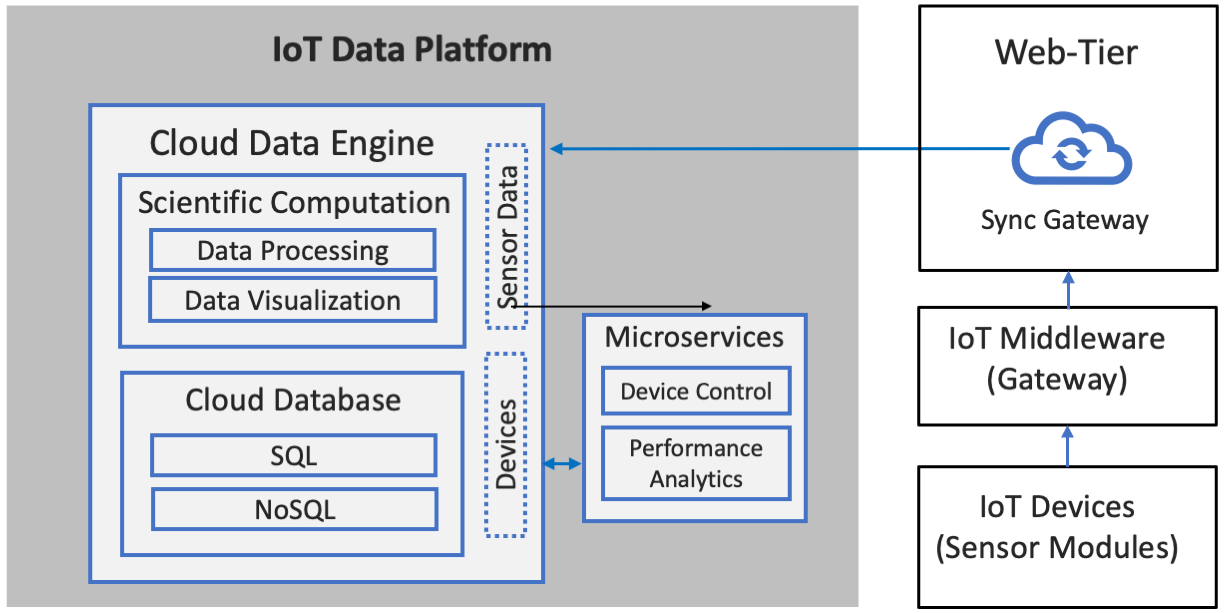
\includegraphics[width=250pt]{fig0.png}
\caption{Proposed Architecture of IoT Data Platform}
\label{fig0}
\end{figure}

The Cloud Data Engine is an integrated server application that runs continuously ingesting as well as processing the incoming data flow. The Cloud Data Engine is connected with the Web-Tier synchronous gateway through MQTT protocol, which can subscribe and publish to the data flow. Inside the Cloud Data Engine, two components were provided. 

\begin{itemize}
	\item \textit{Scientific Computation Module}\\
	The scientific computation module handles and processes the sensor data, which is the ECG data from the edge devices. The scientific computation module is designed as a Plug-in bundle that runs heterogeneous computation tasks on the incoming data flow, produces the expected data outcome, and pushes the results to the corresponding destination i.e. feeding the data to the real-time data visualization.

	\item \textit{Cloud Database}\\
	The cloud databases are the database systems that run on a storage server that stores the incoming data flow simultaneously as the data being processed. The PostgreSQL (relational database) is used for storing the system data i.e. the system configuration data for the sensors. And the MongoDB (NoSQL) is used for storing the sensor data for the sake of improving the network performance.

\end{itemize}

The Microservices component is implemented on the back-end server between the cloud data engine and web-tier application (Sync Gateway), which includes two parts namely, the Device Control component and Performance Analytics component. The Microservices are called on-demand, which are provided with API endpoints and can be accessed using standard HTTP protocol. The Device Control component offers an approach to manage and control the connected devices, such as terminating the devices and fetching the device status \cite{b10}. And the Performance Analytics component can keep track of the network traffic, delay time and resource utilization of the system \cite{b11}.

% When presenting your design, make sure you connect the design with the goals.  In other words, you need to answer the question how this design meets the funtionality requirement and the goals.  This has to be tone for the entire Sec. III and IV.

% (TODO: INSERT FLOWCHART/SEQUENCE DIAGRAM)

% (Sensor $\rightarrow$ Sync Gateway $\rightarrow$ IoT Data Platform $\rightarrow$ Data Processing + Database)

\subsection{Data Flow}\label{DF}

To fullfill the system requirement of real-time data transmission, effective transmission of data flow is proposed in Fig. \ref{dataflow}. The data flow is implemented with two-way communication between the edge and the cloud. The IoT devices can publish the sensor data on a specific topic through MQTT protocol \cite{b12}. Then the MQTT broker will forward and transmit the data to the IoT Data Platform through the Sync Gateway. Then the IoT Platform will store the sensor data in the Cloud Database (NoSQL) and transmit the sensor data to the Scientific Computation Module simultaneously. Furthermore, the sensor data will be sent to the Data Processing component and after data process task is finished, the processed data will be fed into the Data Visualization component and visualize the data using Data Driven Document (D3). Similarly, the IoT devices can also subscribe to a specific topic which allows device control from the cloud (Microservices) to the edge. Each stage of the data flow is transmitted seamlessly from the edge to the cloud through MQTT protocol in real-time \cite{b13}.

\begin{figure}[htbp]
\centering
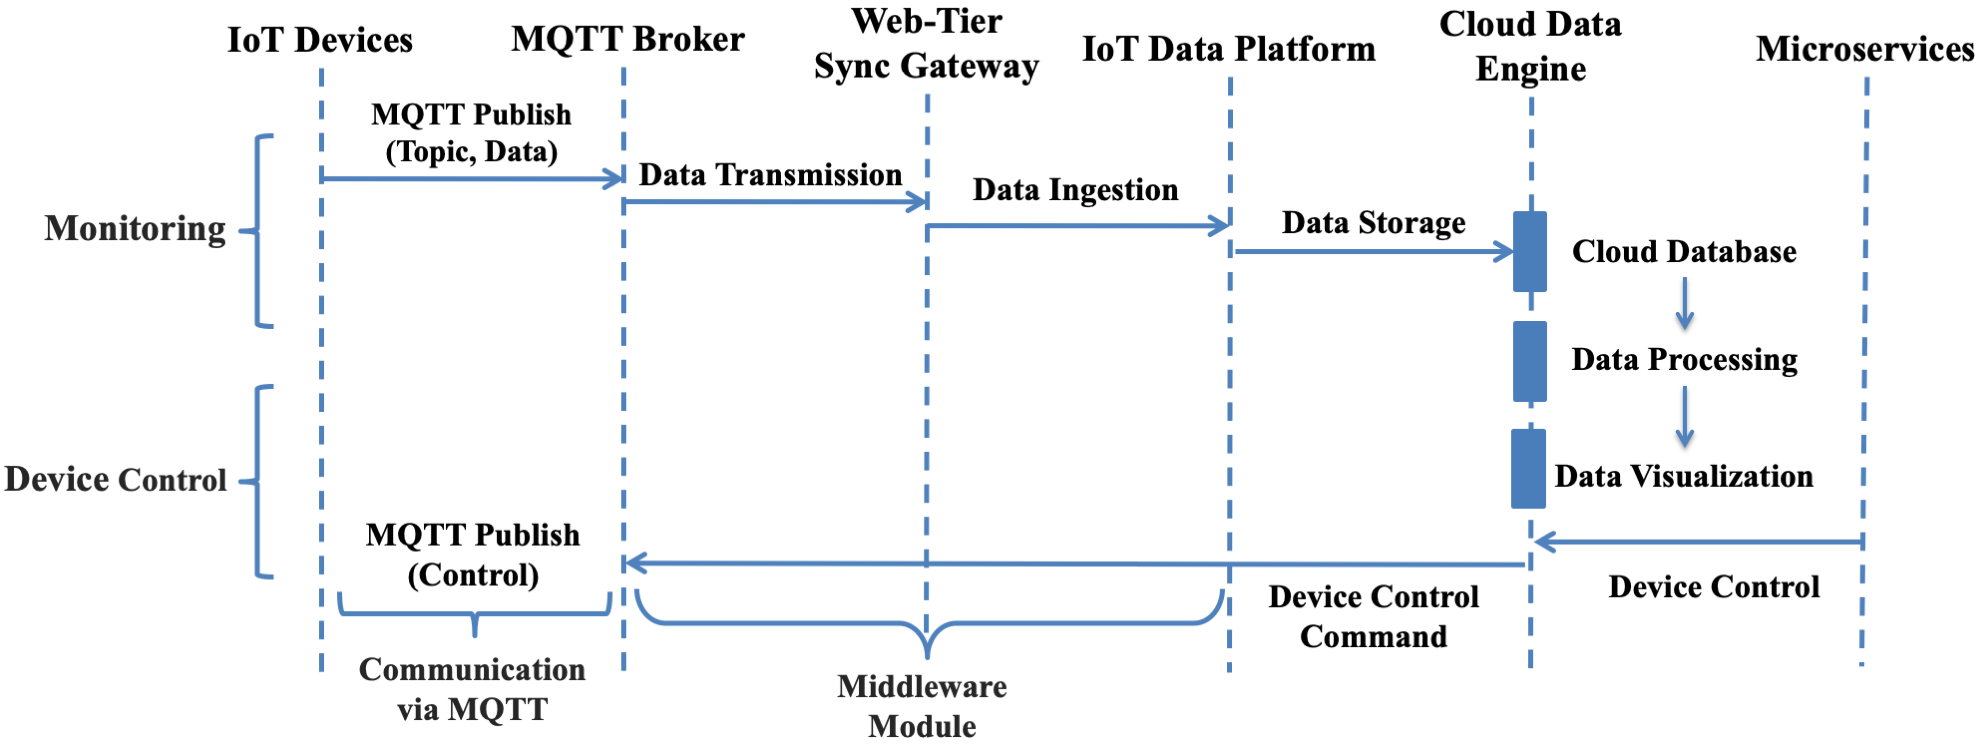
\includegraphics[width=250pt]{dataflow.png}
\caption{Data Flow Sequence Diagram}
\label{dataflow}
\end{figure}




% For Sec 3.1 and Sec 3.2, please focus on the challenges that you need to deal with to meet the system requirement and what is your solution for them.  Please do not just explain your entire implementation without any purpose.


\subsection{Communication Protocols}\label{com}

To achieve the goals of real-time data transmission as well as high concurrency, this paper is utilizing MQTT protocols that can meet the following expectations namely, efficient information distribution, high scalability, reliability, extremely lightweight overhead and reduced network bandwidth consumption \cite{b14}. 

First, MQTT is a publish/subscribe protocol that allows network edge devices to publish to a broker. Clients (IoT Devices) can connect to this broker, which then mediates communication from the edge to the cloud. Each device can subscribe, or register, to particular topics. When another client publishes a message on a subscribed topic, the broker forwards the message to any client that has subscribed. This provides an efficient information distribution for remote sensing and control. Second, the publish/subscribe model is ultra-scalable in an bandwidth-efficient way \cite{b18}. According to HiveMQ \cite{b19}, a HiveMQ broker cluster can support more than 10 million concurrent connections as a distributed system, which scales in a linear fashion and can scale from two cluster nodes up to hundreds. Third, MQTT is bidirectional, and maintains stateful session awareness. If an edge device loses connectivity, all subscribed clients will be notified with the “Last Will and Testament” feature of the MQTT server so that any authorized client in the system can publish a new value back to the edge device, maintaining bidirectional connectivity. In addition, the feature Quality of Service (QoS) options can be used to guarantee data delivery and reliability. Fourth, the extremely lightweight overhead (2-byte header) of MQTT packet makes it possible to significantly increase the amount of data being monitored or controlled.

\subsubsection{MQTT Topic Design}

\begin{figure}[htbp]
\centering
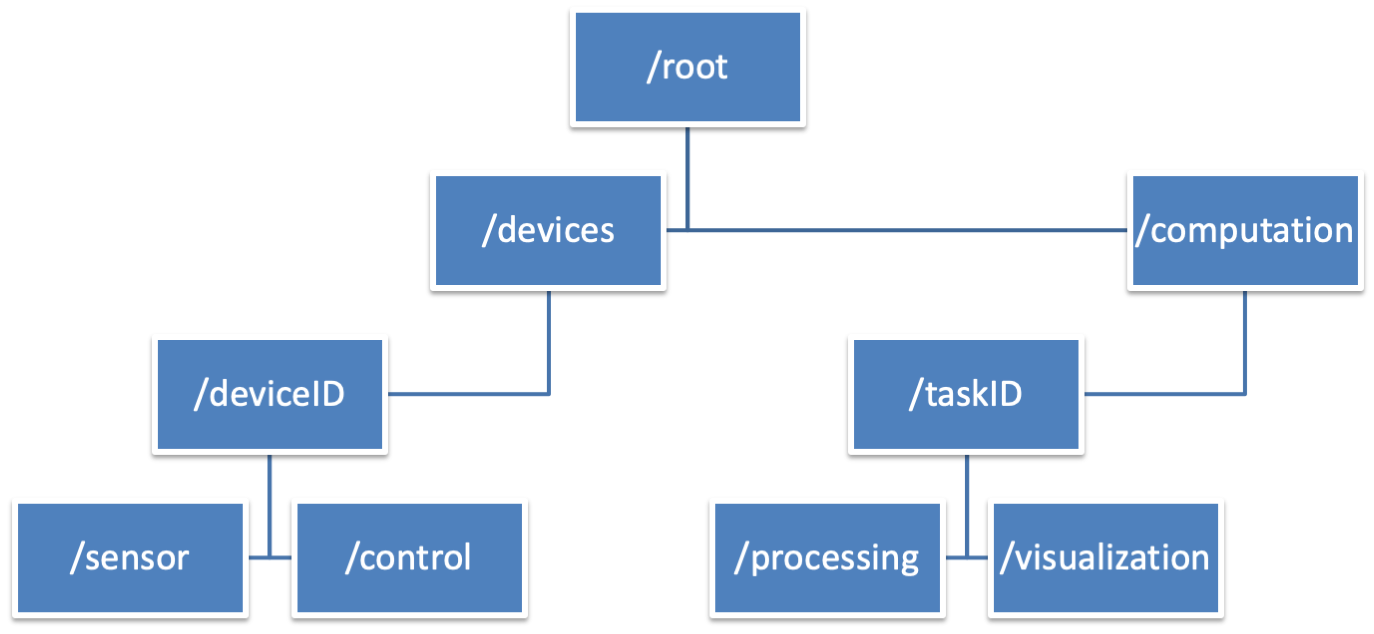
\includegraphics[width=250pt]{topic.png}
\caption{MQTT Topic Hierarchy Design}
\label{topic}
\end{figure}

This paper is proposing a MQTT topic design that is implemented in a hierarchy fasion as shown in Fig. \ref{topic}. The advantage of using the hierarchy design is that it can reduce the system coupling and essentially enhance the system scalability \cite{b15}. The topic start with the root topic '/root' followed by two sub-topics namely, '/devices' and '/computation'. Under the '/devices' topic, the '/deviceID' topic is a universally unique identifier (UUID) which is used to distinguish the connected devices in the system. The '/deviceID' topic has two sub-topics specifically, '/sensor' and '/control', which allows the IoT devices publish the sensor data and subscribe to the device control command respectively. Comparably, under the '/computation' topic, the '/taskID' is also a UUID which is used to differentiate the computation tasks in the Scientific Computation module. The process of the data ingestion, processing and visulization is shown in Fig. \ref{process}. The Data Processing component subscribes to the '/root/devices/deviceID/sensor' topic and creates a computation task processing the incoming data in real-time. Then the Data Visualization component subscribes to the '/root/computation/taskID/processing' to obtain the processed data as well as forward (Publish) the data to an external front-end component (D3) for real-time data visualization.

\begin{figure}[htbp]
\centering
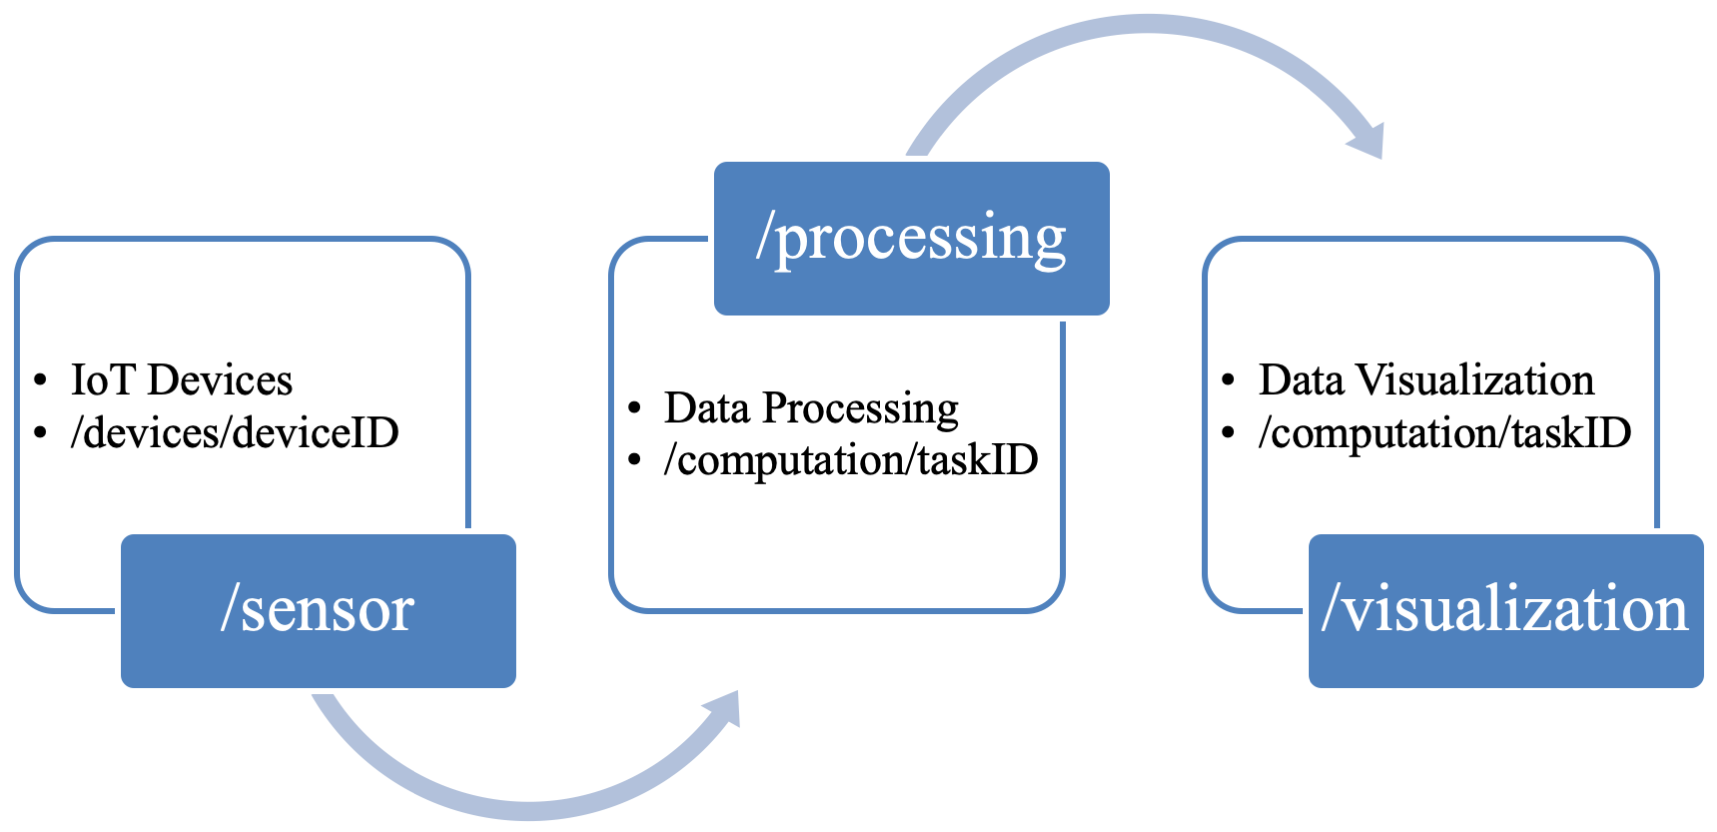
\includegraphics[width=250pt]{process.png}
\caption{Scientific Computation Process}
\label{process}
\end{figure}

\subsubsection{RESTful API Design}

The RESTful API is the endpoints for stateless operations on the Microservices, such as queuing the MQTT server information, controlling the devices and retrieving the performance analytics through standard HTTP protocols.

\begin{figure}[htbp]
\centering
\includegraphics[width=250pt]{packet.png}
\caption{Communication Packet Structure}
\label{packet}
\end{figure}

\subsubsection{Packet Structure}
The packet structure of the sensor data being sent from the edge to the cloud is shown in Fig. \ref{packet}. The packets are sent as an asynchronous serial stream of bytes and each packet begins with its Header, followed by its Data Payload, and ends with the Payload's Checksum Byte. The [PAYLOAD...] section is allowed to be up to 169 bytes long, while each of [SYNC], [PLENGTH], and [CHKSUM] are a single byte each. This means that a complete, valid packet is a minimum of 4 bytes long (possible if the Data Payload is zero bytes long, i.e. empty) and a maximum of 173 bytes long (possible if the Data Payload is the maximum 169 bytes long).



\begin{itemize}
	\item \textit{Packet Header}\\
	The Header of a packet consists of 3 bytes: two synchronization [SYNC] bytes (0xAA 0xAA), followed by a [PLENGTH] (Payload length) byte. The two [SYNC] bytes are used to signal the beginning of a new arriving packet and are bytes with the value 0xAA (decimal 170). And the [PLENGTH] byte indicates the length, in bytes, of the packet's Data Payload [PAYLOAD...] section, and may be any value from 0 up to 169.
	\item \textit{Data Payload}\\
	The Data Payload of a packet is simply a series of bytes. The number of Data Payload bytes in the packet is given by the [PLENGTH] byte from the Packet Header. A DataRow consists of bytes in the following format as shown in Fig. \ref{payload}:
	
	\begin{itemize}
		\item \textit{EXCODE}: The DataRow may begin with zero or more [EXCODE] (Extended Code) bytes, which are bytes with the value 0x55. The number of [EXCODE] bytes indicates the Extended Code Level. The Extended Code Level, in turn, is used in conjuction with the [CODE] byte to determine what type of Data Value this DataRow contains.

		\item \textit{CODE}: The [CODE] byte, in conjunction with the Extended Code Level, indicates the type of Data Value encoded in the DataRow.

		\item \textit{vLength}: A [VLENGTH] ("Value Length") byte immediately follows the [CODE] byte, and this is the number of bytes in [VALUE...].

		\item \textit{value[]}: The arrays of values, i.e. the sensor data.
	
	\end{itemize}

	\item \textit{Payload Checksum}
	The [CHKSUM] Byte must be used to verify the integrity of the packet's Data Payload. The Payload's Checksum is defined as:

	\begin{itemize}
		\item[1.] summing all the bytes of the Packet's Data Payload

		\item[2.] taking the lowest 8 bits of the sum

		\item[3.] performing the bit inverse (one's compliment inverse) on those lowest 8 bits
	
	\end{itemize}

\end{itemize}

\begin{figure}[htbp]
	\centering
	\includegraphics[width=250pt]{payload.png}
	\caption{Communication Packet Payload}
	\label{payload}
	\end{figure}

\subsection{Scalable System Design}

To accomplish the system requirement of high concurrency, this paper chooses to use MQTT protocol to enhance the scalability. However, when using an MQTT protocol, the workload of an MQTT-based system can grow exponentially. The Fig. \ref{mqtt} below explains this concept graphically. For each device ($n$ devices in total), it can choose to talk to the other $n$ devices, which results in the maximum message workload of $n*n=n^2$.

\begin{figure}[htbp]
\centering
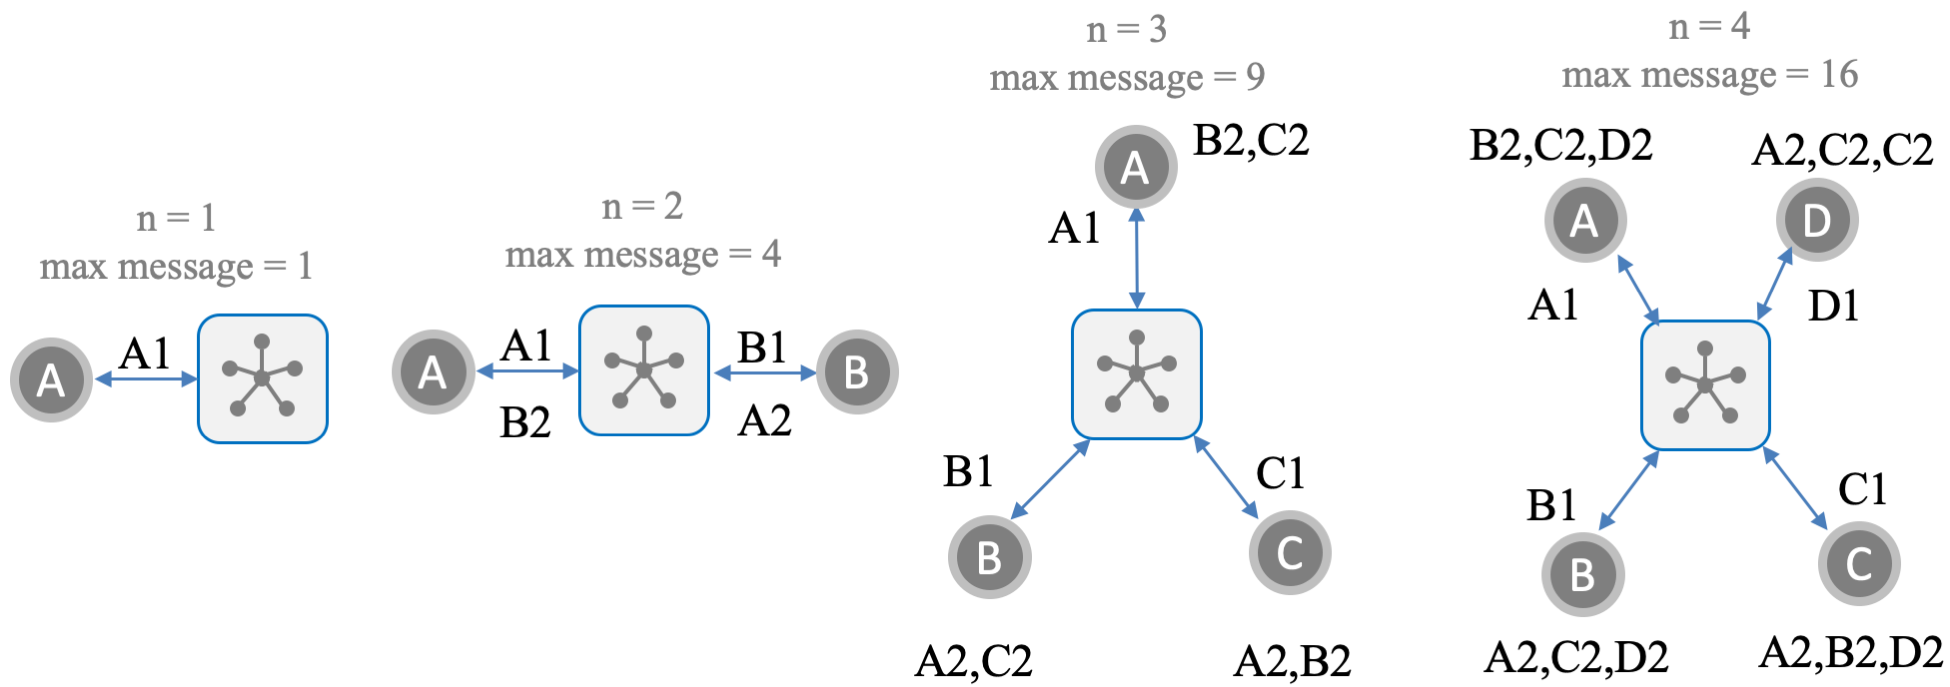
\includegraphics[width=250pt]{mqtt.png}
\caption{Message Workload Grows Exponentially as MQTT Clients Increases}
\label{mqtt}
\end{figure}

\subsubsection{MQTT Broker Cluster}

A scalable MQTT broker cluster is introduced to reduce the workload of the MQTT-based system as well as enhance the scalability of the system. The structure of a scalable MQTT broker cluster is shown in Fig. \ref{loadbalancer}. A MQTT broker cluster is a distributed system that represents one logical MQTT broker. It consists of many different MQTT broker nodes that are typically installed on different physical machines and are connected over a network. From a MQTT client’s perspective, a cluster of brokers behaves like a single MQTT broker. The MQTT Broker Cluster is used in this opioid monitoring system to guarantee the high scalability. Specifically, the IoT devices connect with a broker cluster which is subscribed by the IoT Data Platform. Inside the IoT Data Platform, the Cloud Database module and Scientific Computation module are subscribed by another broker cluster respectively, which enormously enhance the scalability of the proposedb system.

\begin{figure}[htbp]
\centering
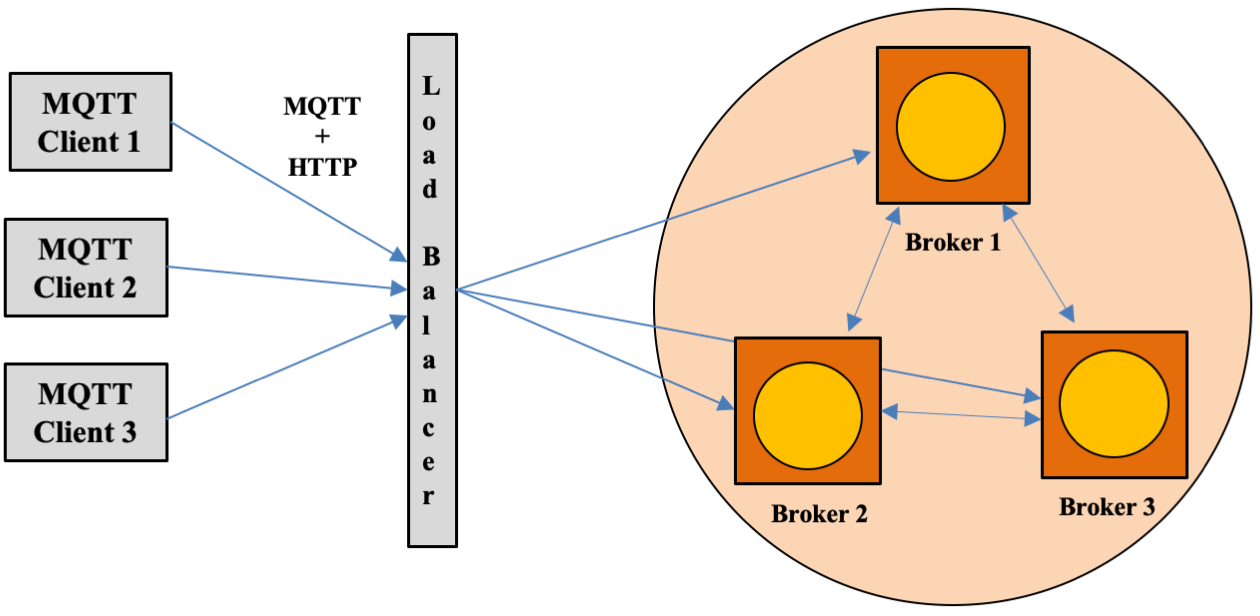
\includegraphics[width=250pt]{loadbalancer.png}
\caption{The Structure of MQTT Broker Cluster}
\label{loadbalancer}
\end{figure}

\subsubsection{Load Balancer}

Load balancers are often used together with MQTT broker clusters to have a single point of entry for all MQTT communication \cite{b16}. In the system implementation, load balancers are used in the entry point of each broker cluster. Any HTTP/TCP load balancer can be used together with any load balancing algorithm below.

\begin{itemize}
		\item \textit{Round Robin (RR)}\\
		A batch of servers are programmed to handle load in a rotating sequential manner. The algorithm assumes that each device is able to process the same number of requests and isn’t able to account for active connections.

		\item \textit{Weighted Round Robin (WRR)}\\
		Servers are rated based on the relative amount of requests each is able to process. Those having higher capacities are sent more requests.

		\item \textit{Least Connections (LC)}\\
		Requests are sent to the server having the fewest number of active connections, assuming all connections generate an equal amount of server load.

		\item \textit{Weighted Least Connections (WLC)}\\
		Servers are rated based on their processing capabilities. Load is distributed according to both the relative capacity of the servers and the number of active connections on each one.
	
	\end{itemize}



This paper proposes a dynamic load balancing algorithm which can switch to different algorithms according to different scenarios. For the initialization stage, the load balancing algorithm is simply Round Robin due to low number of connections. Then if the number of the current connections surpasses the threshold $T$, then it will switch to Weighted Round Robin (Least Connections) algorithm.


\begin{algorithm}
\label{alg}
\caption{Dynamic Load Balancing Algorithm}
\LinesNumbered 
\KwIn{A threshold $T$ of the number of connections}
\KwOut{The broker entry point}

$PriorityQueue \leftarrow Q$;

$Bool \leftarrow INIT$;

$Array \leftarrow Brokers$;

\While{New connections}{

	\If{INIT == TRUE}{
		Run Round Robin algorithm;

		\If{Number of connections $>$ T}{
			$INIT \leftarrow FALSE$;
		}
	}\Else{

		\If{Q.Empty == TRUE}{
			$Brokers \leftarrow HTTPGet()$;
		}

		\ForEach{$broker \in Brokers \ and \  broker \notin Q$}{
			$Q.push(broker)$;  	
	  	}
	  	$return\ Q.pop()$;
	}
}

\end{algorithm}

The Algorithm. \ref{alg} will do HTTP Request (Get) through the RESTful API endpoints to obtain the information of the brokers and uses Priority Queue to keep track of the number of the connections of each broker. If the Priority Queue is using Self-Balancing Binary Search Tree, the time complexity to construct a binary tree is $O(nlogn)$, and the time complexity of adding and deleting is $O(logn)$. Therefore, the average time complexity if $O(logn)$. The advantage of using such dynamic load balancing algorithm is that it can increase the resource utilization while reducing the time complexity, and it can prevent the broker from overflowing by an overwhelming amount of incoming connections spike.

\subsection{EDR Algorithm}

\begin{figure}[htbp]
\centering

\includegraphics[width=220pt]{edr.png}
\caption{The Three Stages of a Estimated RR Algorithm}
\label{edr}
\end{figure}

Estimiated Respiratory Rate (RR) Algorithm can be divided into three stages, as illustrated in Fig. \ref{edr}. Two of the stages namely, 'Extraction of Respiratory Signals' and 'RR Estimation', are compulsory whereas 'Fusion of RR Estimations' is optional \cite{b17}. The Data Processing component in the Scientific Computation module is performing the compuation tasks on the input ECG sensor data. The first stage is to extract the QRS wave from the ECG waveform by applying M-order Low-Pass filter \eqref{lp} as well as M-order High-Pass filter \eqref{hp} to remove the noise, where $a_n,b_n$ are the coefficient of the transfer function. And then it will execute the Pan-Thomkins Algorithm \cite{b21} to calculate the heart rate (HR) and estimated respiratory rate (RR) from the input ECG waveform.

\begin{equation}
H_{LP}(z)=\Sigma_{n=0}^Ma_nz^{-n} \label{lp}
\end{equation}
\begin{equation}
H_{HP}(z)=\Sigma_{n=0}^Mb_nz^{-n} \label{hp}
\end{equation}



% 1) Data Processing: To process the sensor data (ECG
% signals) from the edge device. (TODO: flowchart of processing
% & the Pan-Thomkins Algorithm to calculate heart rate and
% respiratory rate)
% 2) Data Visualization: Feeding the data to the Web-Tier
% dashboard application to show the real-time processed data.



\section{Evaluation}

% More details for this section later.  But for now, it is important for you to think of what do you want to evaluation and how results do you expect.  Common evaluation for platform like this are accuracy of functionalities, resource utilization (especially when the traffic and data volume grows), and response time (especially when the traffic and data volume grows).

\subsection{Accuracy of the EDR Algorithm}

The result of running the EDR Algorithm on a given data set (PhysioNet Fantasia \cite{b22}) is shown in Table \ref{tedr}.

\begin{table}[htbp]
\centering
\caption{Estimated Respiratory Rate (RR) of EDR Algorithm}
\label{tedr}
\begin{tabular}{|c|c|c|c|c|}
\hline
\textbf{Age} & \textbf{Sex} & \textbf{EST. RR/min} & \textbf{ACT. RR/min} & \textbf{Error/ min} \\ \hline
23 & F & 23 & 20 & 3 \\ \hline
28 & F & 16 & 15 & 1 \\ \hline
30 & M & 19 & 17 & 2 \\ \hline
32 & F & 24 & 18 & 6 \\ \hline
68 & M & 17 & 17 & 0 \\ \hline
\end{tabular}
\end{table}

\subsection{Delay of the MQTT Broker Server}
To test the delay between the MQTT Client and the MQTT Broker Server, we utilized Wireshark \cite{b20} to capture the packets between the device and the broker. The filter used in Wireshark, was the port number of the broker server. From Wireshark we determined that the delay was 73 milliseconds. This can vary as we were using the school wifi network which can cause longer processing delays. The data transmission path is shown in Fig. \ref{delay} and since the broker server is hosted in Ashburn, Virginia which is 2,293 miles away, this can cause higher transmission delay. 

\begin{center}
$d_{prop} = (2000\ miles / 3.0 * 10^8 m/s) \approx 10\ ms * 2 = 20\ ms$.
\end{center}

Since the propagation delay is around 20 ms, but the full delay is 73 ms so the rest of the delay is from $d_{queue}$, $d_{trans}$ and $d_{proc}$. There are 30 hops between the MQTT Client and the MQTT Broker server so the queuing delay will be higher. Since the delay of sending and receiving a packet is 73 ms, so just sending would be approximately 36.5 ms. Therefore the sending rate is 1000 ms / 36.5 ms = 27 packets per second.

\begin{figure}[htbp]
\centering
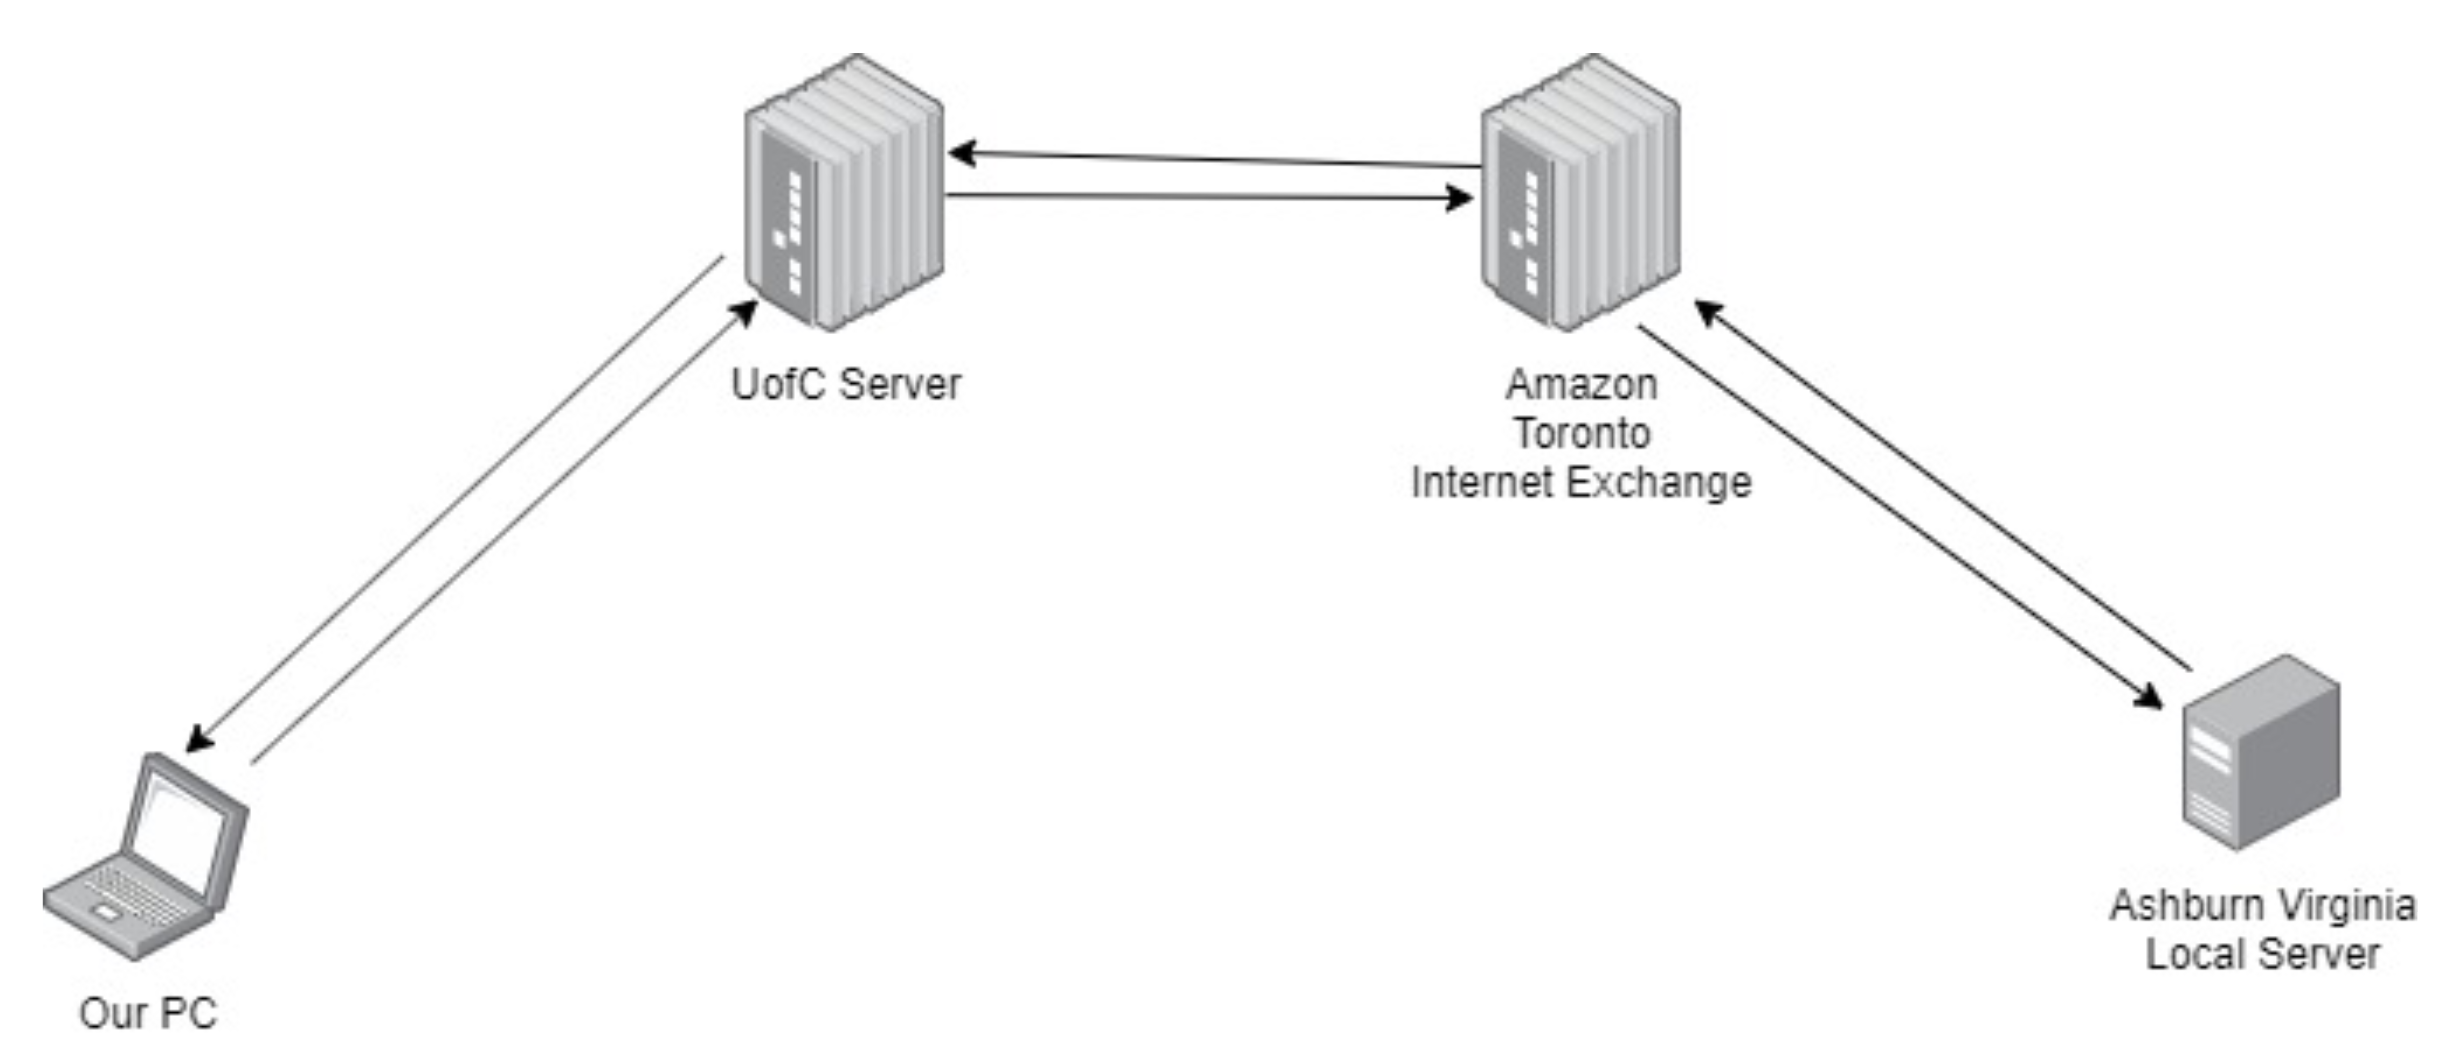
\includegraphics[width=250pt]{delay.png}
\caption{The Data Transmission Path of Sending and Receiving}
\label{delay}
\end{figure}


\subsection{MQTT Broker Server Scalability}
A network analysis tool was used to measure the following metric namely, Throughput, Latency, and Packets Dropped \cite{b20}. For an experimental comparison, a logarithmic scale of clients was chosen to send 1, 10, 100, and 1000 consecutive messages with a reliability of Quality of Service: QoS-0 and QoS-1 in each case. QoS-2 was excluded in test cases due to its large overhead. Table \ref{rst} represents different test case scenarios indicating that the system was able to accept 1000 concurrent MQTT clients publishing messages to a subscribed topic of a single MQTT broker server. From the results as shown in Table \ref{rst}, it is evident that the overall latency for QoS-0 is always lower than that for QoS-1 irrespective of the number of concurrent client requests.

\begin{table}[htbp]
\centering
\caption{MQTT Test Cases and Results}
\label{rst}
\begin{tabular}{ccccccc}
\hline
\textbf{\begin{tabular}[c]{@{}c@{}}Client\\ Number\end{tabular}} &
  \multicolumn{2}{c}{\textbf{Throughput (kbps)}} &
  \multicolumn{2}{c}{\textbf{Latency (ms)}} &
  \multicolumn{2}{c}{\textbf{\begin{tabular}[c]{@{}c@{}}Packets \\ Dropped (\%)\end{tabular}}} \\
      & QoS-0 & QoS-1 & QoS-0 & QoS-1 & QoS-0 & QoS-1 \\ \hline
1     & 2     & 2.6   & 37    & 38    & 0     & 0     \\
10    & 3.6   & 3.9   & 66    & 78    & 0     & 0     \\
100   & 3.5   & 4.9   & 70    & 74    & 0     & 0     \\
1000  & 105.5 & 57.9  & 92    & 112   & 2.9   & 2.6   \\
10000 & 124.3 & 101.5 & 126   & 135   & 3.1   & 3.8   \\ \hline
\end{tabular}
\end{table}

Similarly, another network analysis with the same metric has been measured with a MQTT Broker Cluster of 10 brokers using Round Robin load balancing algorithm. Table \ref{rst2}, Fig. \ref{throughput} and Fig. \ref{latency} present a result that the MQTT Broker Cluster of 10 brokers approximately increase the capacity by a $log_{10}^{10}$ scale. That is because the Round Robin load balancing algorithm spread the work load evenly into 10 brokers compared to a single broker.

\begin{table}[htbp]
\centering
\caption{MQTT Broker Cluster with Load Balancing}
\label{rst2}
\begin{tabular}{ccccccc}
\hline
\textbf{\begin{tabular}[c]{@{}c@{}}Client\\ Number\end{tabular}} &
  \multicolumn{2}{c}{\textbf{Throughput (kbps)}} &
  \multicolumn{2}{c}{\textbf{Latency (ms)}} &
  \multicolumn{2}{c}{\textbf{\begin{tabular}[c]{@{}c@{}}Packets \\ Dropped (\%)\end{tabular}}} \\
      & QoS-0 & QoS-1 & QoS-0 & QoS-1 & QoS-0 & QoS-1 \\ \hline
1     & 1.9   & 2.7   & 35    & 36    & 0     & 0     \\
10    & 2.0   & 2.9   & 41    & 48    & 0     & 0     \\
100   & 2.1   & 3.3   & 45    & 52    & 0     & 0     \\
1000  & 5.0   & 5.7   & 71    & 73    & 0     & 0     \\
10000 & 108.9 & 61.2  & 88    & 107   & 2.9   & 2.8   \\ \hline
\end{tabular}
\end{table}

\begin{figure}[htbp]
\centering
\includegraphics[width=250pt]{throughput.png}
\caption{Throughput vs. Number of Clients}
\label{throughput}
\end{figure}

\begin{figure}[htbp]
\centering
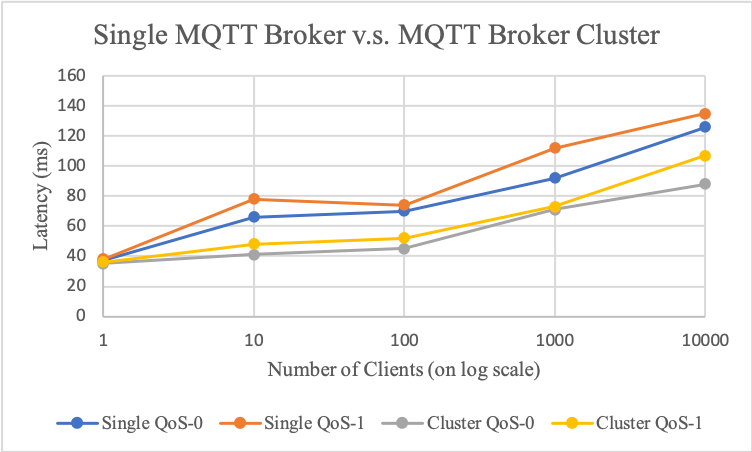
\includegraphics[width=250pt]{latency.png}
\caption{Latency vs. Number of Clients}
\label{latency}
\end{figure}


\subsection{Resource Utilization}

Many users were simulated concurrently using a Webserver Stress Tool on the back-end server which is hosted on Heroku. Each user in this test makes a HTTP GET Request involving retrieving the information from the relational database. CPU and Network utilization were high when all requests started coming as shown in Fig. \ref{rsc}. Almost all requests were answered immediately up to 4000 users. Beyond 4000 users the communication was terminated due to data traffic congestion and testing tool limitation.

\begin{figure}[htbp]
\centering
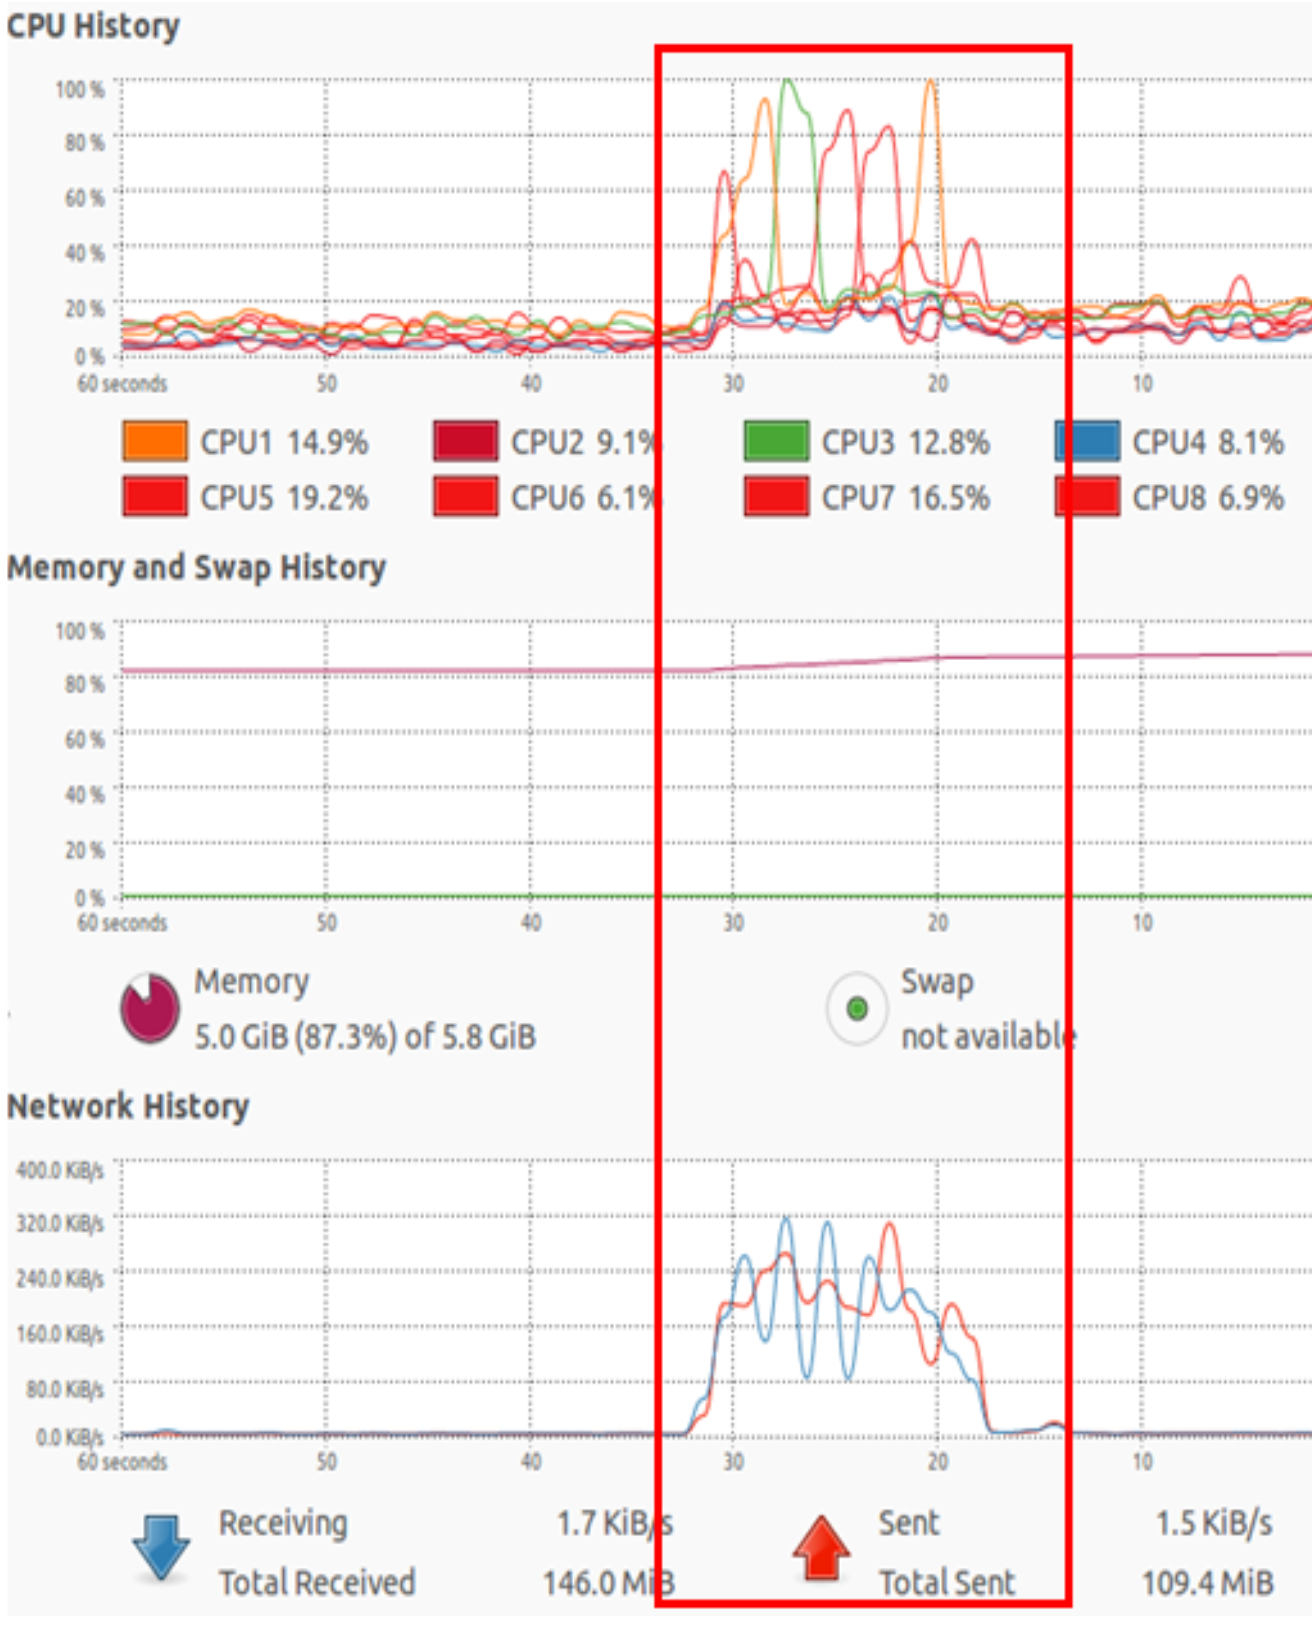
\includegraphics[width=250pt]{rsc.png}
\caption{Server Performance During Request Phase}
\label{rsc}
\end{figure}

\subsection{Response Time}

\begin{table}[htbp]
\centering
\caption{Response Time For 4000 Concurrent Requests}
\label{http}
\begin{tabular}{|c|c|}
\hline
Maximum response time & 322.382 \\ \hline
Average response time & 165.925 \\ \hline
Minimum response time & 080.329 \\ \hline
\end{tabular}
\end{table}

The tested results of HTTP GET Request response time of simulating 4000 cuncurrent users are shown in Table \ref{http}.


\section{Conclusion}

Internet of Things (IoT) has been rapidly developed in the last few years and is increasingly impacting various sectors especially in health monitoring. The proposed work in this paper is to develop an IoT-Based Opioid Overdose Monitoring System as there has been a spike in opioid overdose related deaths, triggering a Public Health Emergency in some provinces, including Alberta. The high scalability and the real-time health monitoring of the proposed system in this paper can help the PWUD reduce the risk of opioid-related deaths, which will not only ease the burden of the opioid epidemic on our healthcare system but also on the lives of those affected.




\newpage

\begin{thebibliography}{00}
\bibitem{b1} Paulozzi LJ, Weisler RH, Patkar AA. A national epidemic of unintentional prescription opioid overdose deaths: how physicians can help control it. J Clin Psychiatry. 2011; 72(5): 589-592. https://doi.org/10.4088/JCP.10com06560 PMID: 21536000
\bibitem{b2} Rudd RA, Aleshire N, Zibbell JE, Gladden RM. Increases in drug and opioid overdose deaths in the United States, 2000±2014.MMWRMorb Mortal Wkly Rep. 2016; 64(50±51): 1378±1382. https://doi.org/10.15585/mmwr.mm6450a3 PMID: 26720857
\bibitem{b3} Ahmad F, Rossen L, Spencer M, Warner M, Sutton P. Provisional drug overdose death counts. Atlanta, Georgia: National Center for Health Statistics, Centres for Disease Control and Prevention, 2018. Available from: https://www.cdc.gov/nchs/nvss/vsrr/drug-overdose-data.htm.
\bibitem{b4} Case A, Deaton A. Rising morbidity and mortality in midlife among white non-Hispanic Americans in the 21st century. Proc Natl Acad Sci USA. 2015; 112(49): 15078±15083. https://doi.org/10.1073/pnas.1518393112 PMID: 26575631

\bibitem{b5} Hall, Wayne D., and Michael Farrell. "Reducing the Opioid Overdose Death Toll in North America." PLoS Medicine 15.7 (2018): E1002626. Web.

\bibitem{b6} Davidson, Peter J, Eliza Wheeler, James Proudfoot, Ronghui Xu, and Karla D Wagner. "Naloxone Distribution to Drug Users in California and Opioid-related Overdose Death Rates." Drug and Alcohol Dependence 156 (2015): E54. Web.

\bibitem{b7} Bratberg, Jeffrey, Bill McLaughlin, and Scott Brewster. "Opioid Overdose Prevention." Journal of the American Pharmacists Association : JAPhA 55.5 (2015): 470-76. Web.

\bibitem{b8} Walley, Alexander Y, Maya Doe-Simkins, Emily Quinn, Courtney Pierce, Ziming Xuan, and Al Ozonoff. "Opioid Overdose Prevention with Intranasal Naloxone among People Who Take Methadone." Journal of Substance Abuse Treatment 44.2 (2013): 241-47. Web.

\bibitem{b9} Clark, Angela, Erin L Winstanley, Donna S Martsolf, and Michael Rosen. "Implementation of an Inpatient Opioid Overdose Prevention Program." Addictive Behaviors 53 (2016): 141-45. Web.

% references from the proposal
\bibitem{ref5}N. Foundation, “Node.js,” Nodejs.org, 2016. [Online]. Available: https://nodejs.org/en/.

\bibitem{ref6}Xu, L. D., He, W. \& Li, S. (2014), “Internet of Things in Industries: A Survey”, Industrial Informatics, IEEE Transactions on 10(4), 2233-2243.

\bibitem{ref7}Yang, G., Xie, L., Mantysalo, M., Zhou, X. L., Pang, Z. B., Xu, L. D., Kao-Walter, S., Chen, Q. \& Zheng, L. R. (2014), “A Health-IoT Platform Based on the Integration of Intelligent Packaging, Unobtrusive Bio-Sensor, and Intelligent Medicine Box”, Industrial Informatics, IEEE Transactions on 10(4), 2180-2191.

\bibitem{ref8}Cho, Wei-Ting, Lai, Ying-Xun, Lai, Chin-Feng, and Huang, Yueh-Min. "Appliance-Aware Activity Recognition Mechanism for IoT Energy Management System." The Computer Journal 56.8 (2013): 1020-1033. Web.

\bibitem{ref9}Man, Lee Carman Ka, Cheng Mei Na, and Ng Chun Kit. "IoT-Based Asset Management System for Healthcare-Related Industries." International Journal of Engineering Business Management 7 (2015): International Journal of Engineering Business Management, 20 November 2015, Vol.7. Web.

\bibitem{ref10}Al-Ali, A. R, Imran A Zualkernan, Mohammed Rashid, Ragini Gupta, and Mazin Alikarar. "A Smart Home Energy Management System Using IoT and Big Data Analytics Approach." IEEE Transactions on Consumer Electronics 63.4 (2017): 426-34. Web.

% \bibitem{ref11}Bell, "Internet of Things Solution", [Online]. Available: https://business.bell.ca/shop/medium-large/internet-of-things

% \bibitem{ref2}Burton, B. \& Willis, D. A. (2014), Gartner’s Hype Cycle Special Report for 2014, Gartner, Inc., pp. 1-11.


\bibitem{b10} Abdelgawad, Ahmed, and Kumar Yelamarthi. "Internet of Things (IoT) Platform for Structure Health Monitoring." Wireless Communications and Mobile Computing 2017 (2017): 10. Web.

\bibitem{b11} Meng, Xiao Jing J., Huan Qing Q. Cui, and Rong Hua. "An IoT-based Remote Health Monitoring and Management System." Applied Mechanics and Materials 571-572 (2014): 1176-179. Web.

\bibitem{b12} Thirunavukkarasu, Gokul, Benjamin Champion, Ben Horan, Mehdi Seyedmahmoudian, and Alex Stojcevski. "IoT-Based System Health Management Infrastructure as a Service." Proceedings of the 2018 International Conference on Cloud Computing and Internet of Things (2018): 55-61. Web.

\bibitem{b13} Yang, Yang, Xianghan Zheng, and Chunming Tang. "Lightweight Distributed Secure Data Management System for Health Internet of Things." Journal of Network and Computer Applications 89 (2017): 26-37. Web.

\bibitem{b18} P. Jutadhamakorn, T. Pillavas, V. Visoottiviseth, R. Takano, J. Haga and D. Kobayashi, "A scalable and low-cost MQTT broker clustering system," 2017 2nd International Conference on Information Technology (INCIT), Nakhonpathom, 2017, pp. 1-5.

\bibitem{b19}HiveMQ, “Creating highly available and ultra-scalable MQTT clusters”. [Online]. Available: https://www.hivemq.com/blog/clustering-mqtt-introduction-benefits/.


\bibitem{b14} Rathore, M., Mazhar Ahmad, Awais Paul, Anand Wan, and Jiafu Zhang. "Real-time Medical Emergency Response System: Exploiting IoT and Big Data for Public Health." Journal of Medical Systems 40.12 (2016): 1-10. Web.

\bibitem{b15} Daeil Kwon, M., Hodkiewicz, Jiajie Fan, Shibutani, and Pecht. "IoT-Based Prognostics and Systems Health Management for Industrial Applications." IEEE Access 4 (2016): 3659-670. Web.

\bibitem{b16} L. Jiang, L. D. Xu, H. Cai, Z. Jiang, F. Bu and B. Xu, "An IoT-Oriented Data Storage Framework in Cloud Computing Platform," in IEEE Transactions on Industrial Informatics, vol. 10, no. 2, pp. 1443-1451, May 2014.

\bibitem{b21} J. Pan and W. J. Tompkins, "A Real-Time QRS Detection Algorithm," in IEEE Transactions on Biomedical Engineering, vol. BME-32, no. 3, pp. 230-236, March 1985.

\bibitem{b22} GOLDBERGER A L, AMARAL L A, GLASS L, et al. PhysioBank, PhysioToolkit, and PhysioNet: Components of a New
Research Resource for Complex Physiologic Signals [J]. Circulation, 2000, 101(23): 215-220.

\bibitem{b20} “Wireshark Go Deep.” Wireshark.org, 2016. [Online]. Available:https://www.wireshark.org/.

\bibitem{b17} Charlton P.H., Villarroel M., Salguiero F. (2016) Waveform Analysis to Estimate Respiratory Rate. In: Secondary Analysis of Electronic Health Records. Springer, Cham.


% \bibitem{b18}
% \bibitem{b19}
% \bibitem{b20}
% \bibitem{b21}
% \bibitem{b22}
% \bibitem{b23}
\end{thebibliography}

% \vspace{12pt}
% \color{red}
% IEEE conference templates contain guidance text for composing and formatting conference papers. Please ensure that all template text is removed from your conference paper prior to submission to the conference. Failure to remove the template text from your paper may result in your paper not being published.

\end{document}


% IoT devices generate an enormous amount of data that need to be stored and processed efficiently. Due to the complexity of the unstructured data generated by IoT devices, it is difficult to organize and process the data. Besides, due to the overwhelming amount of IoT devices, it is impossible to manage them without an efficient management system which can help the individuals collect, organize and transmit the data automatically and efficiently. The data that are collected by the devices can be accessed and processed by the relevant individuals for data analysis or data visualization. Therefore, the data should be stored in a reliable database so that the data can easily be accessed with secure data transmission and access control. Thus, this project will focus on building a management system that will can transmit, store, organize and process the data efficiently and securely.

% The proposed system will be able to transmit, store and manage both the device-generated data and the system data using different databases. More specifically, the device-generated data are normally unstructured and require high-performance demands and flexibility so they will be stored in NoSQL database. Meanwhile, the system configuration data are normally pre-set and well structured so they will be stored in relational database.

% Users will be able to access the data using the provided front-end interface. Also, device data and status can be manipulated as well through the front-end interface. Since there will be potentially a lot of IoT data stored and integrated, the system will allow users to perform specific data processing tasks on the fly. The system will also provide encryption for communication and data transmission between the edge and the cloud.

% \begin{itemize}
% \item Use either SI (MKS) or CGS as primary units. (SI units are encouraged.) English units may be used as secondary units (in parentheses). An exception would be the use of English units as identifiers in trade, such as ``3.5-inch disk drive''.
% \item Do not mix complete spellings and abbreviations of units: ``Wb/m\textsuperscript{2}'' or ``webers per square meter'', not ``webers/m\textsuperscript{2}''. Spell out units when they appear in \item Avoid combining SI and CGS units, such as current in amperes and magnetic field in oersteds. This often leads to confusion because equations do not balance dimensionally. If you must use mixed units, clearly state the units for each quantity that you use in an equation. 
% text: ``. . . a few henries'', not ``. . . a few H''.
% \item Use a zero before decimal points: ``0.25'', not ``.25''. Use ``cm\textsuperscript{3}'', not ``cc''.)
% \end{itemize}

% \subsection{Equations}

% Number equations consecutively. To make your equations more compact, you may use the solidus (~/~), the exp function, or appropriate exponents. Italicize Roman symbols for quantities and variables, but not Greek symbols. Use a long dash rather than a hyphen for a minus sign. Punctuate equations with commas or periods when they are part of a sentence, as in:

% \begin{equation}
% a+b=\gamma\label{eq}
% \end{equation}

% Be sure that the symbols in your equation have been defined before or immediately following the equation. Use ``\eqref{eq}'', not ``Eq.~\eqref{eq}'' or ``equation \eqref{eq}'', except at the beginning of a sentence: ``Equation \eqref{eq} is . . .''

% \subsection{\LaTeX-Specific Advice}

% Please use ``soft'' (e.g., \verb|\eqref{Eq}|) cross references instead
% of ``hard'' references (e.g., \verb|(1)|). That will make it possible
% to combine sections, add equations, or change the order of figures or
% citations without having to go through the file line by line.

% Please don't use the \verb|{eqnarray}| equation environment. Use
% \verb|{align}| or \verb|{IEEEeqnarray}| instead. The \verb|{eqnarray}|
% environment leaves unsightly spaces around relation symbols.

% Please note that the \verb|{subequations}| environment in {\LaTeX}
% will increment the main equation counter even when there are no
% equation numbers displayed. If you forget that, you might write an
% article in which the equation numbers skip from (17) to (20), causing
% the copy editors to wonder if you've discovered a new method of
% counting.

% {\BibTeX} does not work by magic. It doesn't get the bibliographic
% data from thin air but from .bib files. If you use {\BibTeX} to produce a
% bibliography you must send the .bib files. 

% {\LaTeX} can't read your mind. If you assign the same label to a
% subsubsection and a table, you might find that Table I has been cross
% referenced as Table IV-B3. 

% {\LaTeX} does not have precognitive abilities. If you put a
% \verb|\label| command before the command that updates the counter it's
% supposed to be using, the label will pick up the last counter to be
% cross referenced instead. In particular, a \verb|\label| command
% should not go before the caption of a figure or a table.

% Do not use \verb|\nonumber| inside the \verb|{array}| environment. It
% will not stop equation numbers inside \verb|{array}| (there won't be
% any anyway) and it might stop a wanted equation number in the
% surrounding equation.

% \subsection{Some Common Mistakes}\label{SCM}
% \begin{itemize}
% \item The word ``data'' is plural, not singular.
% \item The subscript for the permeability of vacuum $\mu_{0}$, and other common scientific constants, is zero with subscript formatting, not a lowercase letter ``o''.
% \item In American English, commas, semicolons, periods, question and exclamation marks are located within quotation marks only when a complete thought or name is cited, such as a title or full quotation. When quotation marks are used, instead of a bold or italic typeface, to highlight a word or phrase, punctuation should appear outside of the quotation marks. A parenthetical phrase or statement at the end of a sentence is punctuated outside of the closing parenthesis (like this). (A parenthetical sentence is punctuated within the parentheses.)
% \item A graph within a graph is an ``inset'', not an ``insert''. The word alternatively is preferred to the word ``alternately'' (unless you really mean something that alternates).
% \item Do not use the word ``essentially'' to mean ``approximately'' or ``effectively''.
% \item In your paper title, if the words ``that uses'' can accurately replace the word ``using'', capitalize the ``u''; if not, keep using lower-cased.
% \item Be aware of the different meanings of the homophones ``affect'' and ``effect'', ``complement'' and ``compliment'', ``discreet'' and ``discrete'', ``principal'' and ``principle''.
% \item Do not confuse ``imply'' and ``infer''.
% \item The prefix ``non'' is not a word; it should be joined to the word it modifies, usually without a hyphen.
% \item There is no period after the ``et'' in the Latin abbreviation ``et al.''.
% \item The abbreviation ``i.e.'' means ``that is'', and the abbreviation ``e.g.'' means ``for example''.
% \end{itemize}
% An excellent style manual for science writers is \cite{b7}.

% \subsection{Authors and Affiliations}
% \textbf{The class file is designed for, but not limited to, six authors.} A 
% minimum of one author is required for all conference articles. Author names 
% should be listed starting from left to right and then moving down to the 
% next line. This is the author sequence that will be used in future citations and by indexing services. Names should not be listed in columns nor group by affiliation. Please keep your affiliations as succinct as possible (for example, do not differentiate among departments of the same organization).

% \subsection{Identify the Headings}
% Headings, or heads, are organizational devices that guide the reader through 
% your paper. There are two types: component heads and text heads.

% Component heads identify the different components of your paper and are not 
% topically subordinate to each other. Examples include Acknowledgments and 
% References and, for these, the correct style to use is ``Heading 5''. Use 
% ``figure caption'' for your Figure captions, and ``table head'' for your 
% table title. Run-in heads, such as ``Abstract'', will require you to apply a style (in this case, italic) in addition to the style provided by the drop down menu to differentiate the head from the text.

% Text heads organize the topics on a relational, hierarchical basis. For 
% example, the paper title is the primary text head because all subsequent 
% material relates and elaborates on this one topic. If there are two or more 
% sub-topics, the next level head (uppercase Roman numerals) should be used 
% and, conversely, if there are not at least two sub-topics, then no subheads 
% should be introduced.

% \subsection{Figures and Tables}
% \paragraph{Positioning Figures and Tables} Place figures and tables at the top and 
% bottom of columns. Avoid placing them in the middle of columns. Large 
% figures and tables may span across both columns. Figure captions should be 
% below the figures; table heads should appear above the tables. Insert 
% figures and tables after they are cited in the text. Use the abbreviation 
% ``Fig.~\ref{fig}'', even at the beginning of a sentence.

% \begin{table}[htbp]
% \caption{Table Type Styles}
% \begin{center}
% \begin{tabular}{|c|c|c|c|}
% \hline
% \textbf{Table}&\multicolumn{3}{|c|}{\textbf{Table Column Head}} \\
% \cline{2-4} 
% \textbf{Head} & \textbf{\textit{Table column subhead}}& \textbf{\textit{Subhead}}& \textbf{\textit{Subhead}} \\
% \hline
% copy& More table copy$^{\mathrm{a}}$& &  \\
% \hline
% \multicolumn{4}{l}{$^{\mathrm{a}}$Sample of a Table footnote.}
% \end{tabular}
% \label{tab1}
% \end{center}
% \end{table}

% \begin{figure}[htbp]
% \centerline{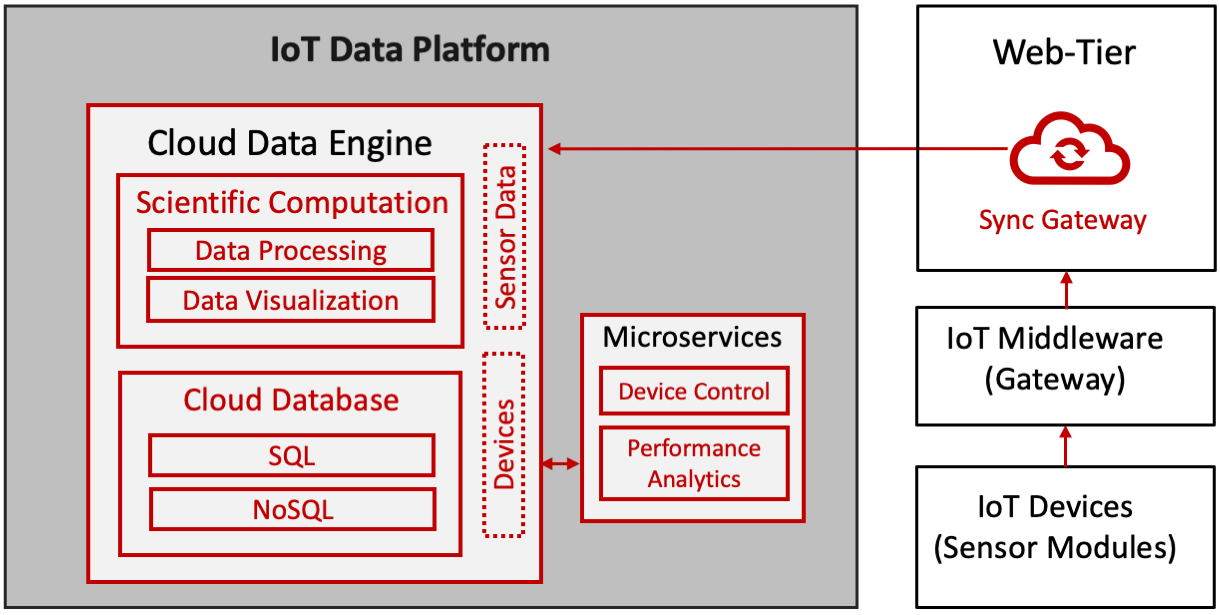
\includegraphics{fig1.png}}
% \caption{Example of a figure caption.}
% \label{fig}
% \end{figure}

% Figure Labels: Use 8 point Times New Roman for Figure labels. Use words 
% rather than symbols or abbreviations when writing Figure axis labels to 
% avoid confusing the reader. As an example, write the quantity 
% ``Magnetization'', or ``Magnetization, M'', not just ``M''. If including 
% units in the label, present them within parentheses. Do not label axes only 
% with units. In the example, write ``Magnetization (A/m)'' or ``Magnetization 
% \{A[m(1)]\}'', not just ``A/m''. Do not label axes with a ratio of 
% quantities and units. For example, write ``Temperature (K)'', not 
% ``Temperature/K''.

% \section*{Acknowledgment}

% The preferred spelling of the word ``acknowledgment'' in America is without 
% an ``e'' after the ``g''. Avoid the stilted expression ``one of us (R. B. 
% G.) thanks $\ldots$''. Instead, try ``R. B. G. thanks$\ldots$''. Put sponsor acknowledgments in the unnumbered footnote on the first page.

% \section*{References}

% Please number citations consecutively within brackets \cite{b1}. The 
% sentence punctuation follows the bracket \cite{b2}. Refer simply to the reference 
% number, as in \cite{b3}---do not use ``Ref. \cite{b3}'' or ``reference \cite{b3}'' except at the beginning of a sentence: ``Reference \cite{b3} was the first $\ldots$''

% Number footnotes separately in superscripts. Place the actual footnote at 
% the bottom of the column in which it was cited. Do not put footnotes in the 
% abstract or reference list. Use letters for table footnotes.

% Unless there are six authors or more give all authors' names; do not use 
% ``et al.''. Papers that have not been published, even if they have been 
% submitted for publication, should be cited as ``unpublished'' \cite{b4}. Papers 
% that have been accepted for publication should be cited as ``in press'' \cite{b5}. 
% Capitalize only the first word in a paper title, except for proper nouns and 
% element symbols.

% For papers published in translation journals, please give the English 
% citation first, followed by the original foreign-language citation \cite{b6}.
